\section{Challenge 3: 1 vs 1}

\subsection{Idea of Challenge}
% Patrick
The aim of this challenge is to have some competitive game play given the current situation.   

This challenge focuses on the following aspects:
\begin{itemize}
    \item Remote or autonomous deployment of NAO software and standardised settings for game play in a remote arena on foreign robots
    \item Automatic and semi-automatic calibration of NAO (vision, motion, etc.) 
    \item One versus One NAO competition in a ladder KO competition with all teams without much robot interaction. 
\end{itemize}

Requirements to participate in the scored part of this challenge are being able to
\begin{itemize}
    \item host an arena
    \item deploy your robot's software remotely or fully autonomous setup. 
\end{itemize}

If teams provide an autonomous setup all teams can use this to play against this in their own arena. Also teams who cannot host an arena.

\subsection{Prerequisites}
% Patrick
For this challenge teams need to fulfil multiple requirements, which are listed below in more detail.

First to be able to participate Teams have to  be able to deploy their software on the NAO remotely or you can deliver an autonomous setup. There will be several opportunities for the teams to talk, discuss, exchange ideas and code over the next few month until RoboCup. Two options will be properly available: Meetings like RoDEO and an spring RoHOW as well as to discuss on the SPL Discord channel. The second option is a code sharing section as it is available for the V6 support on RC SPL website.  

If teams are not able to participate, they (and the other teams as well) can download and deploy the images for fully autonomous setup, calibration and challenge play in the own lab. These games are not part of the ladder system and are outside of the competition.

\subparagraph*{Basic requirements for teams}

\begin{itemize}
    \item A team must be able deploy their robot software remotely or be able to produce a fully autonomous image for a robot
    \item A team must be able to host an arena. If not they have to find an substitute team, who takes over their hosting arena responsibilities.
    \item A robot must be able to semi- or fully automatic calibrate itself
\end{itemize}

\subparagraph*{Basic requirements for arenas}

The following items have to fulfilled to be able to host an arena.

\begin{itemize}
    \item A field that is nearly of the size of a 3/4 field or larger.
    \item Field marks as stated in the rules section. 
    \item Two standard goals with nets.
    \item Wifi with standard SPL\textunderscore A session, standard password and standard IP address and DHCP turned off.
    \item Remote network access via:
    \begin{itemize}
        \item VPN connection
        \item Mobile connection
        \item TeamViewer or remote desktop connection
    \end{itemize}
    \item Camera, tablet or laptop for on field online calibration with remote team using Discord.
    \item Streaming setup to stream the game on YouTube/Discord/BigBlueButton/Zoom ..., what is available (If bandwidth in the lab is limited, an restreaming should be considered on system with better network connection)
    \item Latest Game Controller running.
    \item At least 4 working NAOs V6 per game.
    \item Multiple USB Sticks with 16 GB or more memory  for flashing and logging 
    \item At least 4 balls.
    \item Assistants for remote setup and autonomous setup
    \item Referees
\end{itemize}

\subsection{Arena and organisational setup}
% Patrick
This challenge relies on a standardised arena setup as well as on exchanging all necessary information. This section provides the description for this.

\subsubsection{Data Exchange}
A NextCloud storage is used for data exchange during the days of RoboCup 2021. An access link and password will be sent to the team leaders and have to be used with care. In the NextCloud every team has its own folder (team number) which will be used for sharing the following data:

\begin{itemize}
    \item In folder \textbf{field dimensions} each team has to provide an json file (template will be given) describing the field dimensions according to the rules (TODO: link). The file has to be named \texttt{field\_dimensions.json}. This file has to be uploaded until the 15th of June 2021. The file will be used for autonomous setup and game play. To configure the arena the corresponding field dimensions json will be copied next to the image on the robot as field\_dimensions.json. This allows the usage of the same image at different arenas.
    TODO: Define Json (team name, necessary fields, wifi 2.4 or 5)
    \item  In the folder \textbf{field images} each team has a folder where photos from the arena from different angles and at different day \& night times with focus on the lighting conditions get uploaded until the 15th of June 2021.
    \item In \textbf{Robot Setup} the arena teams find an image for a particular game. Each game has an identifier and this identifier should be used as folder name. The image has to be uploaded \textbf{two hours} before the game starts.
    \item In \textbf{Arena Access} remote teams find an instruction how to access the arena. It has to contain all necessary information including usernames,  passwords or certificates. This folder in only shared with SPL teams.
    \item In the root folder you find a \texttt{streaming.md} file where every team should publish a link that can be used by public to watch the game.
    \item Logs and Images will be uploaded from the hosts into the folder \texttt{Logs/Game\_ID}, where \textit{Game\_ID} is replaced by the game identifier, after the game when bandwidth is available. It is assumed that Logs and images are stored on the USB drive attached to the NAO in the folder \texttt{logs}. Other files will be ignored.
\end{itemize}

\subsubsection{Network Setup}
The following section defines network requirements for a venue that hosts remote games. The network infrastructure should be as transparent as possible for remote participants. It should get as close as possible to an on-site experience.

\paragraph{General}

\begin{itemize}
    \item Participants need easy access to their robots for uploading code and debugging. No ports should be blocked. ICMP must not be blocked.
    \item Robots might accumulate a large amount of log files (including images). These logs are generally downloaded after games for analysis. Minimum 500Mbit/s (symmetric) is recommended for a venue, favorable 1Gbit/s.
    \item To not overwhelm the network, teams should rate limit their network activity (in particular long log downloads and uncompressed video streams from NAOs during debug sessions)
\end{itemize}

\paragraph{SPL Game specific}

\begin{itemize}
    \item Team Messages (SPLStandardMessages) must be receivable for remote participants
    \item Team Messages must not be forwarded from remote participants to 10.0.0.0/16 (SPL\_A)
    \item GameControllerMessages must be receivable for remote participants
    \item GameControllerMessages must not be forwarded from remote participants to 10.0.0.0/16 to not allow remote participants to control the game (by accident)
\end{itemize}

\paragraph{Example configuration}

\begin{figure}[ht!]
    \centering
    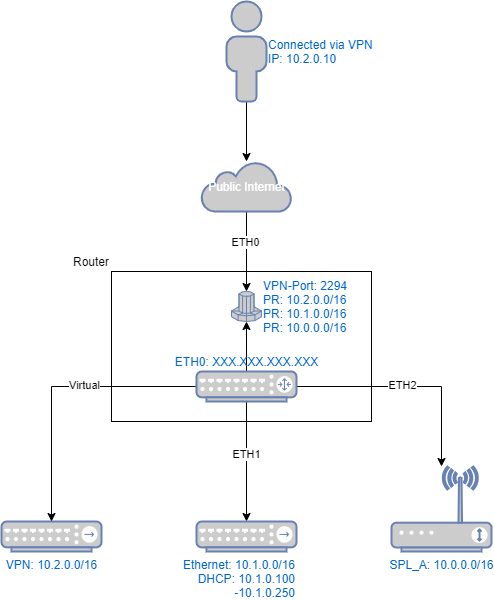
\includegraphics[width=0.5\textwidth]{figs/network.png}
    \caption{Network setup example}
\end{figure}

\begin{itemize}
    \item  The network is divided into three subnets:
    \begin{itemize}
        \item 10.0.0.0/16: The actual SPL\_A wifi network. Each team must use 10.0.TEAM\_NO.2-254 for their robots. GameController will be on 10.0.0.2. DHCP is not active.
        \item 10.1.0.0/16: The ethernet network for robots. Each team must use 10.1.TEAM\_NO.2-254 for their robots. Static addressing is required when robots are assigned to a team. DHCP is active, statically assigning 10.1.0.2-255 to robots that are currently not assigned to any team (pool).
        \item 10.2.0.0/16: The VPN network. Remote participants are assigned to this network and can access the other networks. Team- and GameControllerMessages are forwarded from 10.0.0.0/16 to this subnet. DHCP is active. Broadcasting to other subnets is not possible.
    \end{itemize}
    \item Router (e.g. Edge Router line from Ubiquity)
    \begin{itemize}
        \item serves as router for the whole network.
        \item has a globally routable (and accessible) IPv4 address.
        \item hosts an OpenVPN Layer2 VPN Server
        \item opens a network port to allow incoming OpenVPN connections
        \item Every team gets one certificate to authenticate via OpenVPN (multiple connections allowed).
        \item Has broadcast forwarding rules in place to allow VPN users to receive Team-/GC-Messages.
        \item GameController computer is assigned 10.0.0.2/16
        \item \texttt{ETH0} could be connected to your university network and is preferably accessible from the internet on the specific port (please contact your computer centre how to realise such a connection). If this is not possible, please check if you can make this network accessible from remote using a mobile internet connection. Or you provide a PC connected to an island network of this structure were people can access the PC using Teamviewer, remote desktop software, or something similar. 
    \end{itemize}
\end{itemize}

\subsection{Remote \& Game Setup}
    % - https://writemd.rz.tuhh.de/Tu3JCxovRVunD_yZwBl5Vw#
    % - https://writemd.rz.tuhh.de/rQE55j51QzqO98ifHYF0cQ#
    % - https://writemd.rz.tuhh.de/2YL-Gkz7QX2_zeJyD5Y1jA#

\subsubsection{Start: 2h before match}

    \begin{itemize}
        \item For each team two randomly selected robots are assigned from the pool
        \item Connect robot to LAN and power line
        \item Each robot gets flashed 
        \begin{itemize}
            \item with the standard Softbank image and the LAN IP address is set to 10.1.TEAM\_NO.2 and the replacement robot to 10.1.TEAM\_NO.3, if no individual image is provided by the team.
            \item with the image provided by the teams together with the field\_dimension.json and robot\_id.json indicating if the main robot or the replacement robot gets flashed. (TODO: Create json) 
        \end{itemize}
        \item Teams setup robots remotely, if necessary.
    \end{itemize}

\subsubsection{Calibration / Testing: 1 hour before match)}

    \begin{itemize}
        \item 20 min to calibrate the two robots supported by one volunteer from the hosting team. Use for communication the Discord server.
        \item  
    \end{itemize}

    Each team has 1/2 hour on full field for calibration with the help of 1 Volunteer
    Check for wifi
    Check for GC connection

Game setup

    As proposed in special corona rules
    standardized procedure for all teams (Because volunters move robots)
    Referees apply rules to prevent hardware damages (No SBR support probably)
    Longer Pause
    2 preliminary games halfes

Game end

    Teams have 10 min to clear robots (may be longer due to limited internet connection)
    Robots are returned to pool
    Next games start



\subsection{Rules}

\subsubsection{Robot Players}
\label{sec:robot_players}
A match is played by two teams, each consisting of \emph{one player} and \emph{one substitute player}. All robots are \emph{field players} and no robot is designated as \emph{goalkeeper}.

\subsubsection{Hardware}
\label{sec:hardware}
All teams must use black, gray, red, blue, or orange plated NAO humanoid robots manufactured by SoftBank Robotics.

\textcolor{red}{TODO}: enforce V6?

Absolutely no modifications or additions to the robot hardware are allowed. No additional hardware is permitted including off-board sensing or processing systems. Additional sensors besides those originally installed on the robots are likewise not allowed. The only exceptions are:
\begin{itemize}
	\item Setting the passive wrist joints to a fixed position either with glue or a transparent or white duct tape.
	\item Protecting the fingers with white finger protectors provided by the manufacturer or with transparent or white duct tape.
	\item Placing white duct tape over the battery case and screw (under the robot jersey) to keep the battery case in place and prevent the battery becoming disconnected.
	\item A memory stick may remain in the head during operation.  Only ordinary USB flash memory keys that sit flush or recessed to the head casing may be utilized. Other USB dongles or devices, as well as memory sticks that are not flush or recessed, are not permitted.
\end{itemize}

\subsubsection{Field Players}
\label{sec:field_players}
Each field player has a jersey number from the set $\{1, 2, 3, 4, 5, 6\}$. However, by default, the number ``1'' is used for the first field player and the number ``2'' should be used for a substitute that enters the game later. This assignment can be changed due to availability of jerseys.

\subsubsection{Team Markers}
\label{sec:team_markers}
Robots use colored jersey shirts as team markers. Each jersey shirt has a player number (1-6) printed on it. The team markers are worn as shown in Figure~\ref{fig:nao_markers}.

\begin{figure}
	\centerline{\begin{tabular}{lll}
			a) & b) & c) \\
			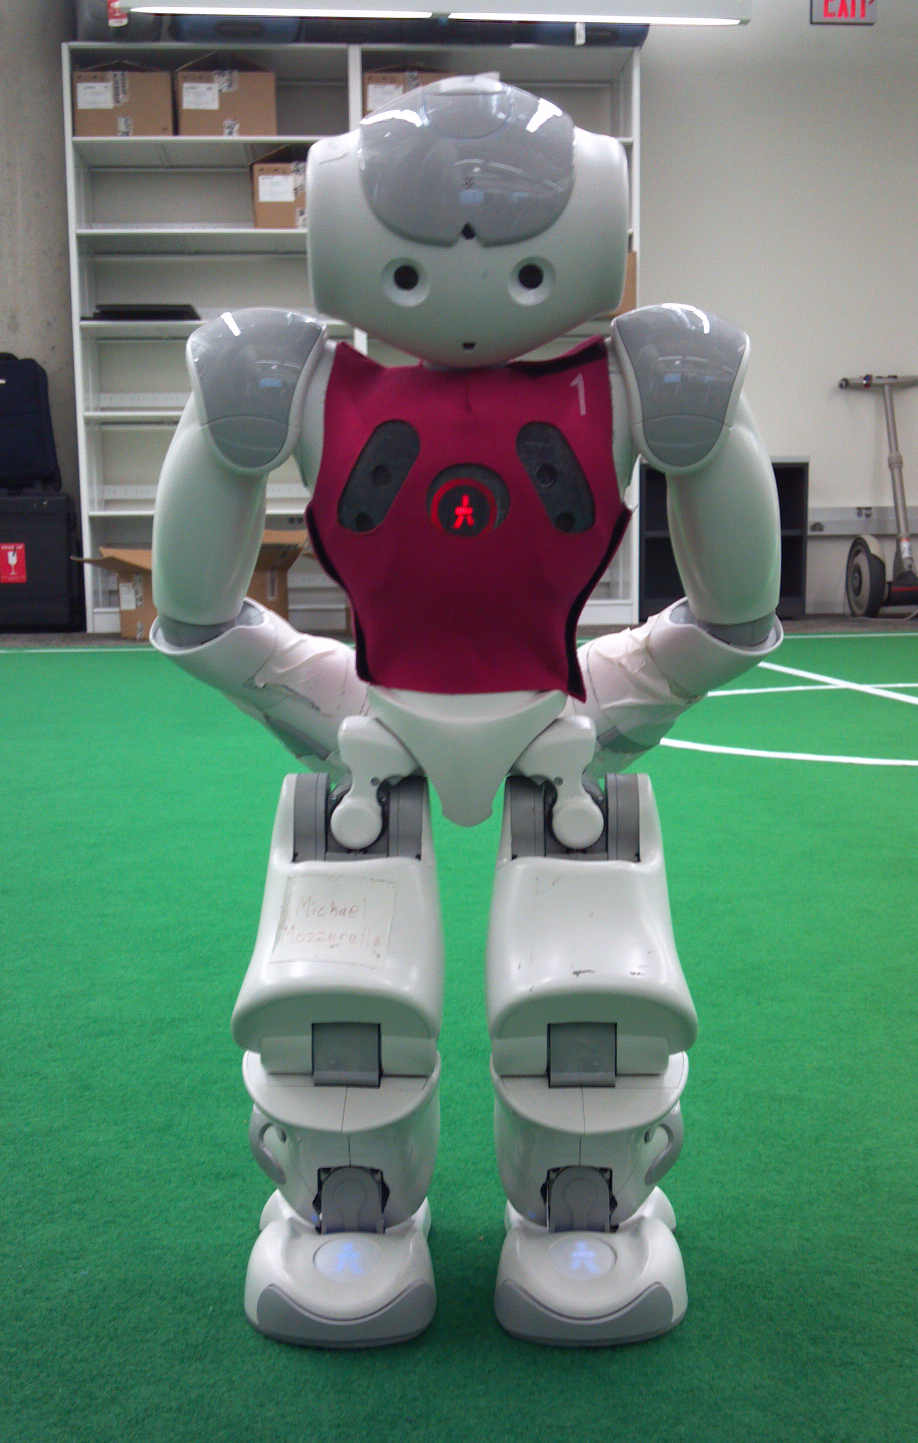
\includegraphics[height=0.28\columnwidth]{figs/front.jpg}&
			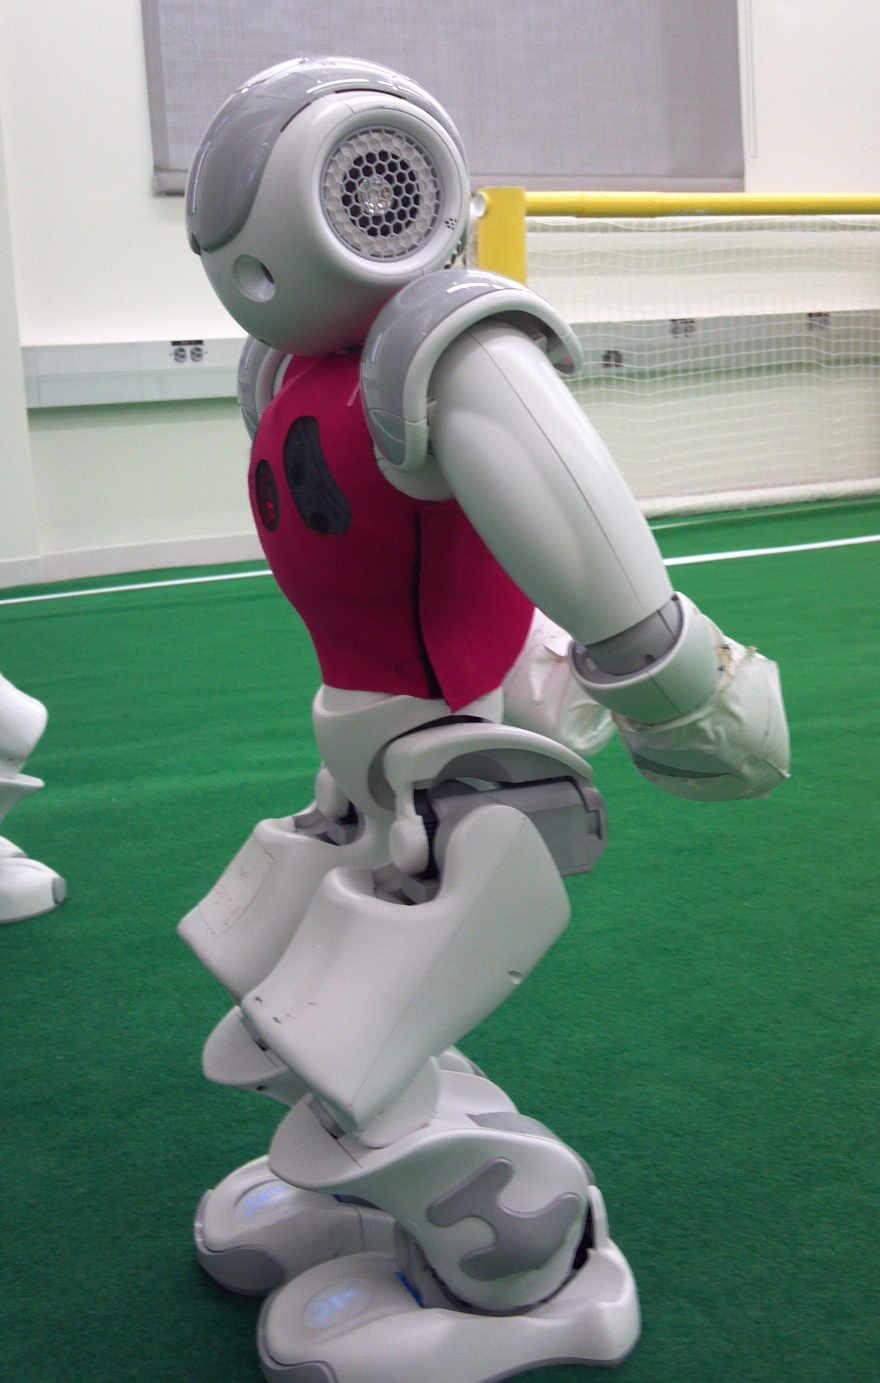
\includegraphics[height=0.28\columnwidth]{figs/side.jpg} &
			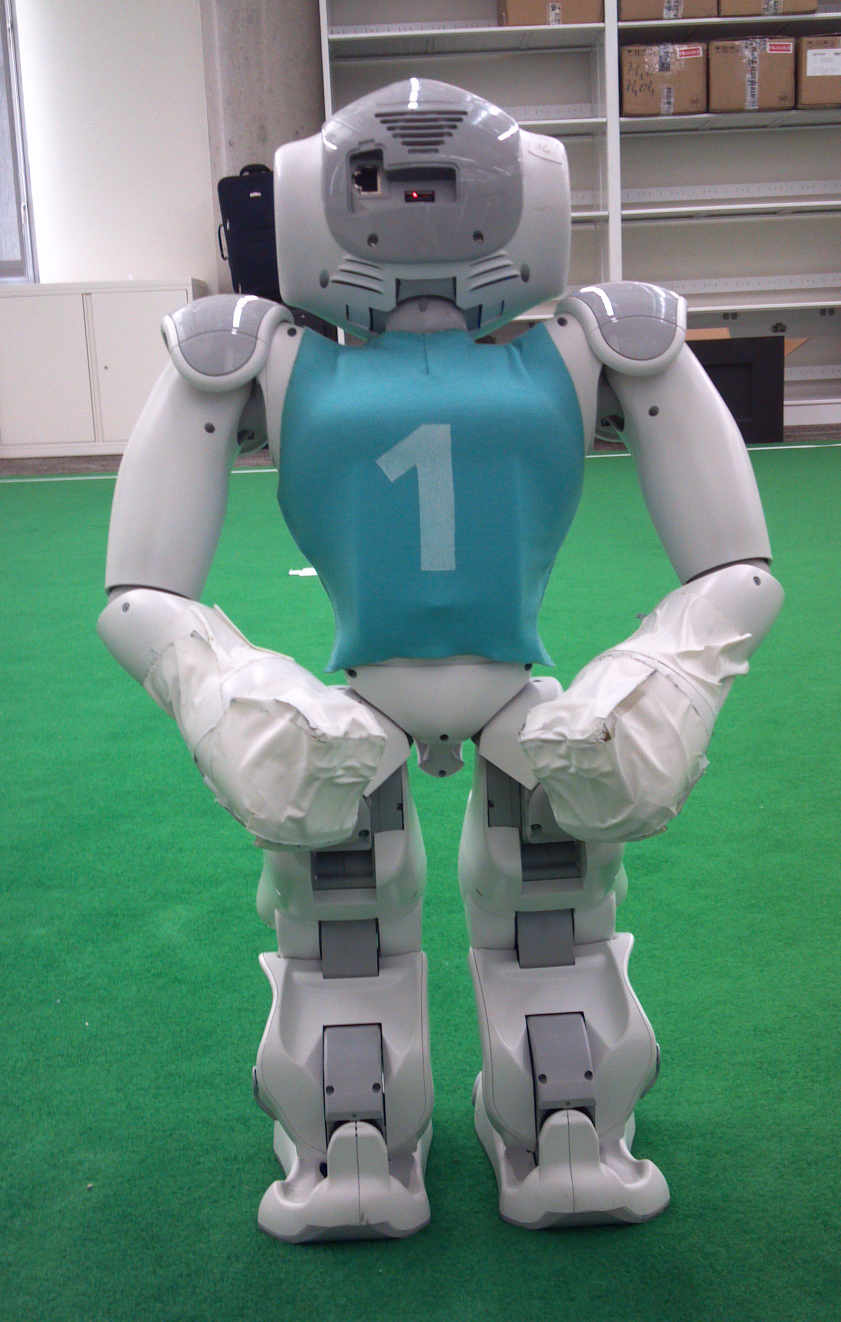
\includegraphics[height=0.28\columnwidth]{figs/back.jpg}
	\end{tabular} }
	\caption{Team markers. a) Front view. b) Side view. c) Back view.}
	\label{fig:nao_markers}
\end{figure}


Teams may design and manufacture their own jerseys in any color (multi and many color jerseys are acceptable), but must follow these guidelines:
\begin{itemize}
	\item Jerseys should be the tank top style used at RoboCup 2013/2014 and should cover approximately the same areas of the robot as shown in Figure~\ref{fig:nao_markers}.  The torso LED must be clearly visible.  Jerseys may include the sonar panel used in the 2013/2014 jerseys, although this is not required.
	\item Jerseys must have a primary color that comprises at least 70\% of the jersey.
	\item Jerseys should not contain distractors, such as large pictures of SPL balls or white stripes on green jerseys.
	\item All players on a team must wear identical jerseys.
	\item A team must wear the jerseys that it starts a game in for the entire game.
	\item Jersey material must be non-reflecting, non-shiny, and non-textured.  Material that is glittery is also not appropriate.
	\item Jerseys should be numbered 1-6 on both sides.  The numbers must be large and {\bf easily} recognized by humans.
	\item Teams must have two sets of jerseys that are significantly different in terms of their primary color.
	\item Designs must be submitted to \url{rc-spl-tc@lists.robocup.org} for approval by May 1, 2021. If the team has jersey prototypes, they should submit close-up images of a robot wearing the jersey - these images should be taken from front, back, and side angles.  If the team has no prototypes, then designs depicting the expected jersey should be submitted.  If submissions show separated front and back halves of jerseys then the team must specify which halves are matched to form home and away jerseys.  All images and designs should be submitted in pdf or jpg format.
\end{itemize}

Each team/arena must designate a `home' color and an `away' color when asked about one month before RoboCup. Robots must wear the `home' jerseys when they are `home' (the first team listed on the schedule). The `away' team (the second team listed on the schedule) will wear the `away' jerseys.

Some teams wish to include additional information or logos on their robots.  The following are allowable:
\begin{itemize}
	\item Attaching player numbers to the heads and/or legs of the robots.  These numbers should be black with a white background, and should correspond to the number on the robot's jersey.
	
	\item Adding sponsor or team logos to the upper legs of the robots (\cf Figure~\ref{fig:sponsor}). A box drawn around the non-white area of these logos must not cover more than a 25 $\text{cm}^2$ area. At most one logo may be attached per leg --- if you wish to attach more than one logo per leg, email the Technical Committee at least two weeks before the competition.  Depending on the size and design of the logos, this may be allowable.
	
	\item Adding small black and white stickers to the torso of the robots stating the name of the robot, the name of the team, or similar information. These stickers must be small and mostly white.
\end{itemize}

\begin{figure}[b]
	\centerline{\begin{tabular}{ll}
			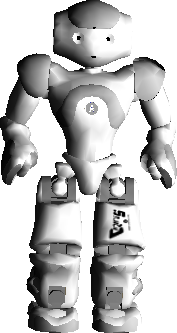
\includegraphics[height=0.35\columnwidth]{figs/naosim_with_logo.png}&
			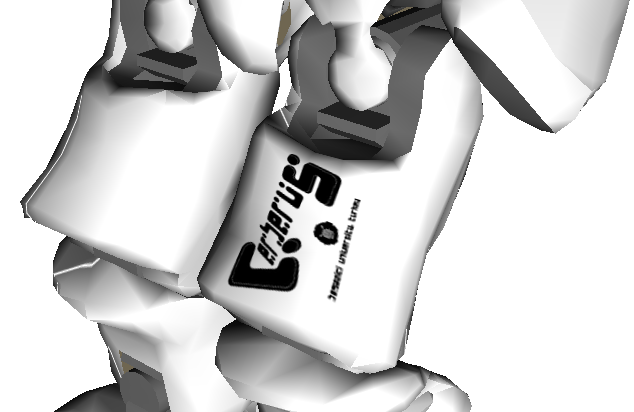
\includegraphics[height=0.35\columnwidth]{figs/naosim_legs_with_logo_closeup.png}
	\end{tabular}}
	\caption{Example Sponsor/Team Logo placement on legs.}
	\label{fig:sponsor}
\end{figure}

\subsubsection{Communications}

The robots must play without human control. Communication is only allowed between a robot and the GameController.

\subsubsection{Wireless Communications}
\label{sec:wireless}
The only wireless hardware allowed to be used by the teams/arenas are the wireless network cards built into the NAOs, and the access points provided by the arena. All other wireless hardware must be deactivated. A team/arena may be disqualified if one of the team members violates this rule.

Each team will get a range of IP addresses that can be used both for their robots and their computers/remote connections. The network configuration (\eg IP addresses, channels, SSIDs, and required encryption) of the fields will be announced by the arena. 

\textcolor{red}{TODO}: add default configuration

Teams and their robots must not listen into another team's communication.

The GameController will use UDP to connect to the robots. The source distribution of the GameController provides the header file \emph{RoboCupGameControlData.h} that defines all messages sent by the GameController to the robots. They correspond to the \emph{robot states} described in Section~\ref{sec:robot_states}.

Robots send status updates (defined in \emph{RoboCupGameControlData.h}) to the GameController. These return packets must be addressed directly to the GameController PC (\ie not broadcast) and sent on the GameController return UDP port specified by the symbol \verb!GAMECONTROLLER_RETURN_PORT! in \emph{RoboCupGameControlData.h}.

The use of remote processing/sensing is prohibited.

\subsubsection{Structure of the Competition}
\label{sec:game_struct}

A 1vs1 competition consists of three parts, the first half, a half-time break, and the second half. Each half is 5 minutes counted from the initial kick-off.
The half-time break is five minutes and during this time both teams may change their robot to the substitute player, but code changes are prohibited in the half-time. It is mainly used to cool down the robots and to charge them. 

The head referee signals the commencement of each half with a single whistle blow (that is, the Initial kick-off, \cf Section~\ref{sec:initial-kick-off}).
The head referee signals the end of the first half with two short whistle blows, and the end of the second half with two short plus one long whistle blow.
The head referee should make \textit{all} of these whistle sounds from the T-junction of the half-way line.

The teams/robots will change the goal defended during the half-time break.

\subsubsection{Robot States}
\label{sec:robot_states}

Robots can be in six different \emph{primary} states (\cf Figure~\ref{fig:robot_states}). If the wireless is available, these states will be set by the GameController. Teams must implement code to receive and correctly respond to wireless GameController packets, and also give a visual indication of the game state.
\emph{If a robot does not respond to the GameController then it is not included in the game (via a `Request for Pick-up'), and the game starts without the offending robot. The use of the button interface is not allowed in this competition.}

\begin{description}
	\item[Initial.] After booting, the robots are in their \emph{initial} state. The robots are not allowed to be moving in any fashion besides initially standing up. Shortly pressing the chest button will switch the robot to the \emph{penalized} state.
	
	\item[Ready.] In this state, the robots walk to a legal position on their half. They remain in this state, until the head referee decides that there is no significant progress, up to a maximum of \KickOffAutoTime.
	
	\item[Set.] In this state, the robots stop and wait for Kick-Off  (\cf Section~\ref{sec:kick-off}).
	Illegally positioned robots are penalized.
	Robots are allowed to move their heads or get up if fallen before the game (re)starts but they are not otherwise allowed to move their legs or locomote in any fashion.
	If a robot cannot get up, fallen robot is called~(\cf Section~\ref{sec:fallenrobots}).
	The penalty time counter is frozen during this state.
	Note that all penalised robots are left in place (on the side of the field, or in-place for motion in set) and must wait to get unpenalized.
	
	\item[Playing.] In the \emph{playing} state, the robots are playing the 1vs1 competition.
	
	\item[Penalized.] A robot is in this state when it has been penalized. It is not allowed to move in any fashion,  this includes stopping the head turning.
	
	\item[Finished.] This state is reached when a half is finished.
\end{description}

\begin{figure}[t]
	\centerline{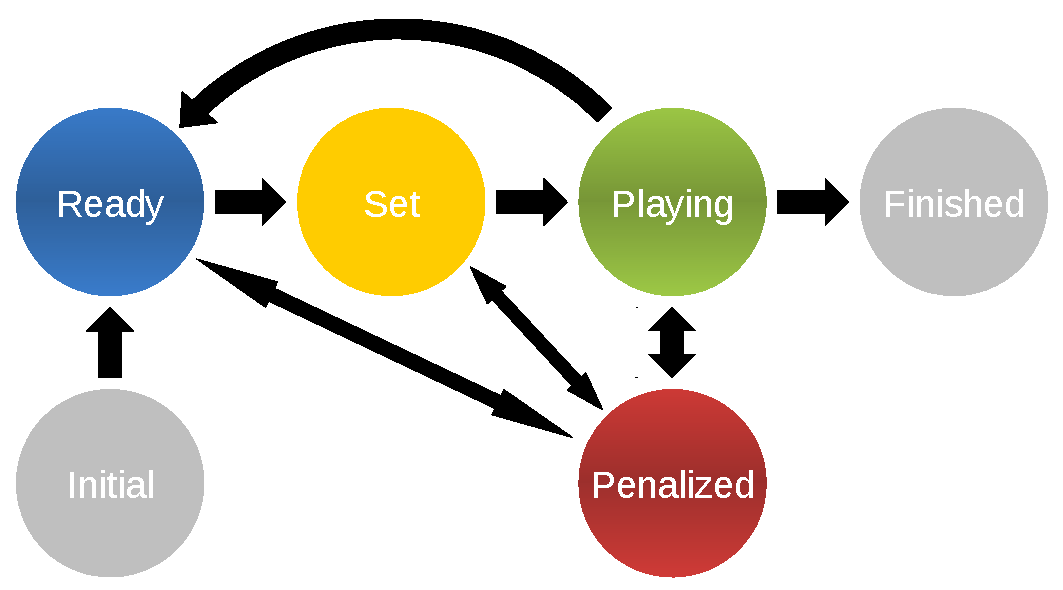
\includegraphics[width=0.9\columnwidth]{figs/states.pdf}}
	\caption{Robot states. GameController transitions are shown in black. However, any transition possible for this competition is only sent by the GameController.}
	\label{fig:robot_states}
\end{figure}

The referee will announce the start of the Playing state with a single whistle blow.
The GameController Playing signal will be delayed by \PlayingDelayTime.
Robots that begin moving their legs or locomoting in any fashion during \emph{set} (\ie before the referee blows the whistle) will be penalized \textit{in place} on the field via the ``Motion in Set'' (\cf Section~\ref{sec:motion_in_set}) GameController signal (and moved back to their original position if they have moved significantly before becoming penalized) until the GameController transmits the \emph{playing signal}.

The current game state should be displayed on the LED in the torso. The colors corresponding to the game states are:

\begin{itemize}
	
	\item Initial: Off
	
	\item Ready: Blue
	
	\item Set: Yellow
	
	\item Playing: Green
	
	\item Penalized: Red
	
	\item Finished: Off
	
\end{itemize}

The current GameController requires robots to know both their team number and their robot number within the team. It is each team's responsibility to make sure this is correctly configured. It is recommended that the robot indicates its number within the team on bootup so that this can be easily checked at the start of the game.

\subsubsection{Goal}
\label{sec:goal}
A goal is achieved when the entire ball (not only the center of the ball) goes over the goal-side edge of the goal line, \ie the ball is completely inside the goal area\footnote{The goal line is part of the field.}. \\
If a player scores a valid goal the ball gets replaced by the referees to one of the starting points, on its own side, that is farthest away from the player. The ball can then directly be played again. 
\textcolor{red}{TODO}: Reference.

\label{sec:invalid_goal}
A goal is invalid (that is, it can never be awarded) when a team scores on themselves.
\textcolor{red}{TODO}: Replacement of the ball by own goal?

The head referee signals a goal by a single whistle blow, followed by the call ``Goal \textless color\textgreater''. However no Gamecontroller action shall be performed. \textcolor{red}{TODO}: Reference. \\
After the game is in the state playing, the game state remains in it regardless of shot goals!


\subsubsection{Initial Kick-off}
\label{sec:initial-kick-off}

The first kick-off at the start of each half is the initial kick-off.
Before the initial kick-off, \ie before the start of each half, both robots must be in the initial state and must be placed on the sidelines, closest to the GameController, in their own half of the field at the height of the penalty spot. 
Once the robots receive the \emph{ready} signal from the GameController, they are to proceed as described in Section~\ref{sec:kick-off}.

\subsubsection{Kick-off}
\label{sec:kick-off}
For kick-off, the robots listen to the wireless GameController and run through three states: \emph{ready}, \emph{set}, and \emph{playing}. It is to a team's responsibilty to have their robots listen to the GameController.

In the ready state, the robots should walk to their legal kick-off positions.
The players can be positioned anywhere within their own half, but no player is allowed to touch the halfway line. All robots that do not reach legal positions will be penalized with the ``Illegal Position'' penalty~(\cf Section~\ref{sec:illegal_positioning}).

In the \emph{set} state, the robots must not locomote~(\cf Section~\ref{sec:robot_states}). A referee places the two balls for each side on the goal free kick positions.\textcolor{red}{TODO}:Reference. If the ball is moved by one of the robots during Set it is replaced by one of the referees.

\textcolor{red}{TODO}:allow manual placement?
%During the \textit{set} state, the team leader may request manual placement for all robots on that team --- including those penalized in place for ``Motion in Set'' but not those with other penalties. Note that the, ``Motion in Set'' penalty persists for those players after manual placement.

%\begin{figure}[t]
%	\centerline{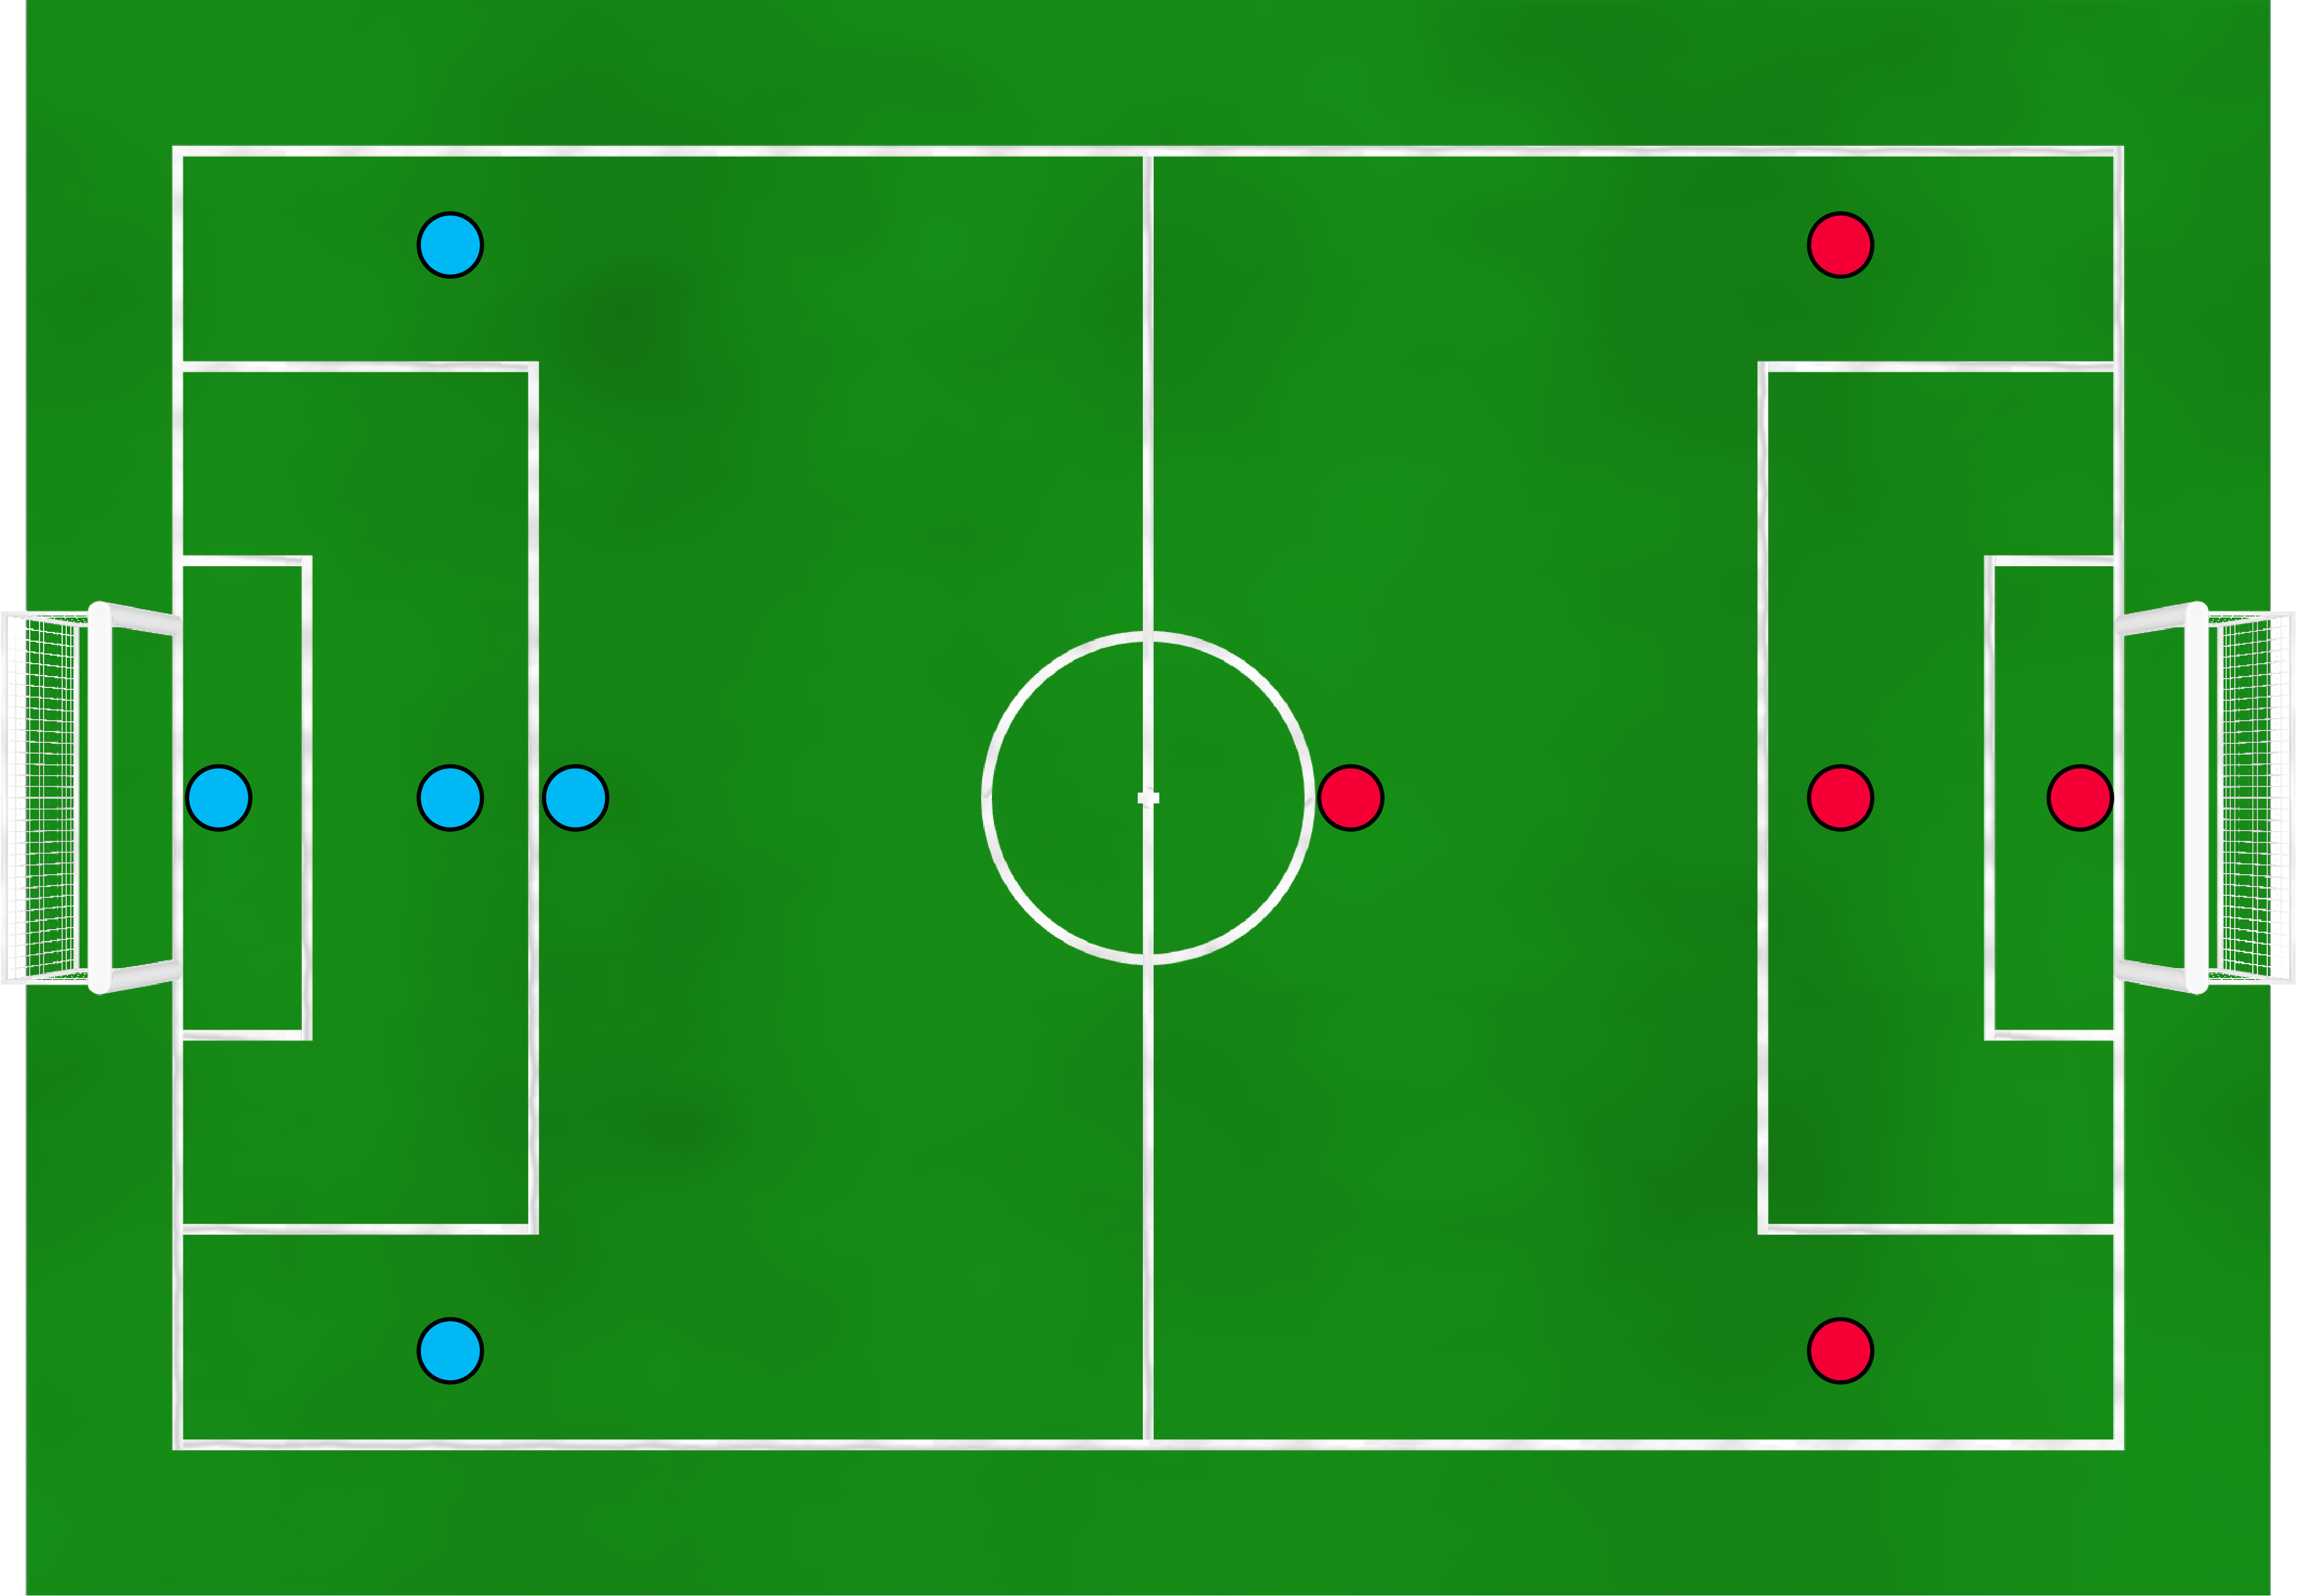
\includegraphics[width=\columnwidth]{figs/manual-placement-2020.png}}
%	\caption{Manual setup for kick-off.  The attacking team is on the right.}
%	\label{fig:ko}
%\end{figure}

%The positions for manually positioned robots are shown in Figure~\ref{fig:ko}. The kicking-off robot is placed such that its feet touch the center circle (but are not inside it), right in front of the penalty mark. The goal keepers for each team are placed at the center of the goal, with their feet immediately in front of the end-line.
%The other robots are positioned relative to the penalty spot, with one robot on the spot, and others outside of the penalty box.

%To assist the referees in placing the robots manually when needed or requested, small Xs will be marked on the field using a black felt-tip pen in the spots where manually placed robots should go.  These marks should be small, such that they are visible to humans but invisible to robots.

The head referee signals the kick-off by a single whistle blow, followed by the call ``Playing''. The head referee must signal this from the T-junction of the half-way line.

After the head referee has signalled the kick-off, the robot's state is switched to \emph{playing} by the GameController.

\subsubsection{Kick-in}
\label{sec:kick_in}

A ball is considered to have left the field when there is no part of the ball over the outside of the boundary line (\ie the line itself is in). \\
If the ball goes over a sideline then the assistant referee will replace the ball back on the point of that sideline where it went out. \\
If the ball goes over an end-line then the assistant referee will replace the ball onto the corner of the Goalbox on the same side of the field that the ball was kicked-out. That is, the corner inside the field, not the t-junction where the goalbox meets the goal line.

\subsubsection{Global Game Stuck}
\label{sec:game_stuck:global}

In the event of no substantial change in the game state for 30 seconds OR or no ball was played onto the other half for 1 minute, this is considered a global game stuck and the referee calls ``Global Game Stuck''. ``Substantial change'' can consist of a robot seeing and moving towards the ball OR robots exploring the field (presumably in an attempt to find the ball). Once the referee calls Global Game Stuck, players enter the Ready state, and a new kick-off (see Section \ref{sec:kick-off}) is awarded.

\subsubsection{Request for Pick-up}
\label{sec:request_for_pickup}

Either team may request that their players be picked up (called ``Request for Pick-up'').
In the Playing or Ready state, players may only be picked up for hardware failures.
In all other states, players may be picked up for any reason.

Only hardware changes are allowed during a request for pick-up. In particular,
it is permitted to change batteries, fix mechanical problems, reboot the robots.
It is also allowed to replace a broken robot by a substitute robot.
It is prohibited to change the robot's control program.

Any strategic ``Request for Pick-up'' is not allowed.
That is, gaining an advantage by removing the robot from the game.
In this case, the head referee will indicate when the robot is no longer affecting play and can be removed from the field by an assistant referee.

To prevent mistakes and confusion during games, only team leaders should make a ``Request for Pick-up''.
The returning robot may be returned following the normal replacement procedure once at least 45 seconds have elapsed since the robot was removed from play.
Note that this penalty does not follow the standard removal procedure, and hence does not count towards the incremental penalty count.
If the picked-up robot was penalized, the penalty time of the robot counts down with the game clock throughout the pick-up.

Note here, that the returning robot or the substitute robot will have to wait out any remaining penalty time of the picked up robot after the team handed their robot back to the assistant referees.

\textcolor{red}{TODO}: RFP because of no Gamecontroller, automatic request for Pickup Referee, Assistants fix Hardware Problems?

\subsubsection{Referee Timeout}
\label{sec:referee_timeout}
The head official may call a timeout at any stoppage of play if he or she deems it necessary.  A referee timeout should only be called in dire circumstances --- one example might be when the power to the wireless router is down or no robot listens to the GameController.  However, when and whether to call a referee timeout is left up to the head referee.

Referees may call multiple timeouts during a game if needed.  Teams are only allowed to do hardware changes during these timeouts.  The referee should end the timeout once he or she believes the circumstance for which the timeout was called has been resolved.  In cases where the circumstance for which the timeout was called is not resolved within 10 minutes, the chair of the technical committee should be consulted regarding when/if play should continue.

\subsubsection{Penalty Procedure}
\label{sec:penalty_procedure}

When a robot commits a foul, the head referee shall call out the infraction committed, the primary jersey color of the robot, and the jersey number of the robot. The penalty for the infraction will be applied immediately by an assistant referee. The assistant referees should perform the actual movement of the robots for the penalty so that the head referee can continue focusing on the game. The operator of the GameController will send the appropriate signal to the robots indicating the infraction committed.

For penalties that are timed, the penalty time is considered to be over at the end of each half.
In general, when a penalty applies, the robot shall be replaced, not the ball.

\subsubsection{Standard Removal Penalty}
\label{sec:removal_penalty}

Unless otherwise stated, all infractions result in the removal of the infringing robot from the field of play for a particular amount of time, after which it will be returned to the field of play. This process is called the \textit{standard removal penalty}.

When the head referee indicates a foul has been committed that results in the standard removal penalty, the assistant referee closest to the robot will remove the robot immediately from the field of play. The robot should be removed in such a way as to minimize the movement other robots and the ball. If the ball is inadvertently moved when removing the robot, the ball should be replaced to the position it was in when the robot was removed.

The GameController will send the appropriate penalty signal to the robot indicating the infraction committed. After a penalty is signalled to the robot, it is not allowed to move in any fashion. The removed robot will be placed outside of the field facing away from the field of play.

The initial duration of the standard removal penalty time is \StandardPenaltyTime.
Unless otherwise specified, the penalty time increases by \StandardPenaltyIncrease each time a team commits any infraction.
That is, the first infraction will result in a penalty time of \StandardPenaltyTime, the second infraction (of any type) results in a penalty time of 55 seconds, the third infraction is 65 seconds, etc.

During the \emph{set} state the penalty time counter will not decrease.

The GameController will keep track of the time of the penalty. The operator of the GameController will signal the assistant referees when the penalty is 10 seconds from being over, so that one of them can place the robot in the half of the field which this robot's team is defending on the sideline that is nearest to the GameController. The robot should be placed close to the position where the penalty spot projects on the sideline. This is illustrated in Figure~\ref{fig:penalty_re-entry_points}.

With approximately 5 seconds left before the penalty ends, the robot should be turned to face towards the opposite sideline.

\begin{figure}[t]
	\centerline{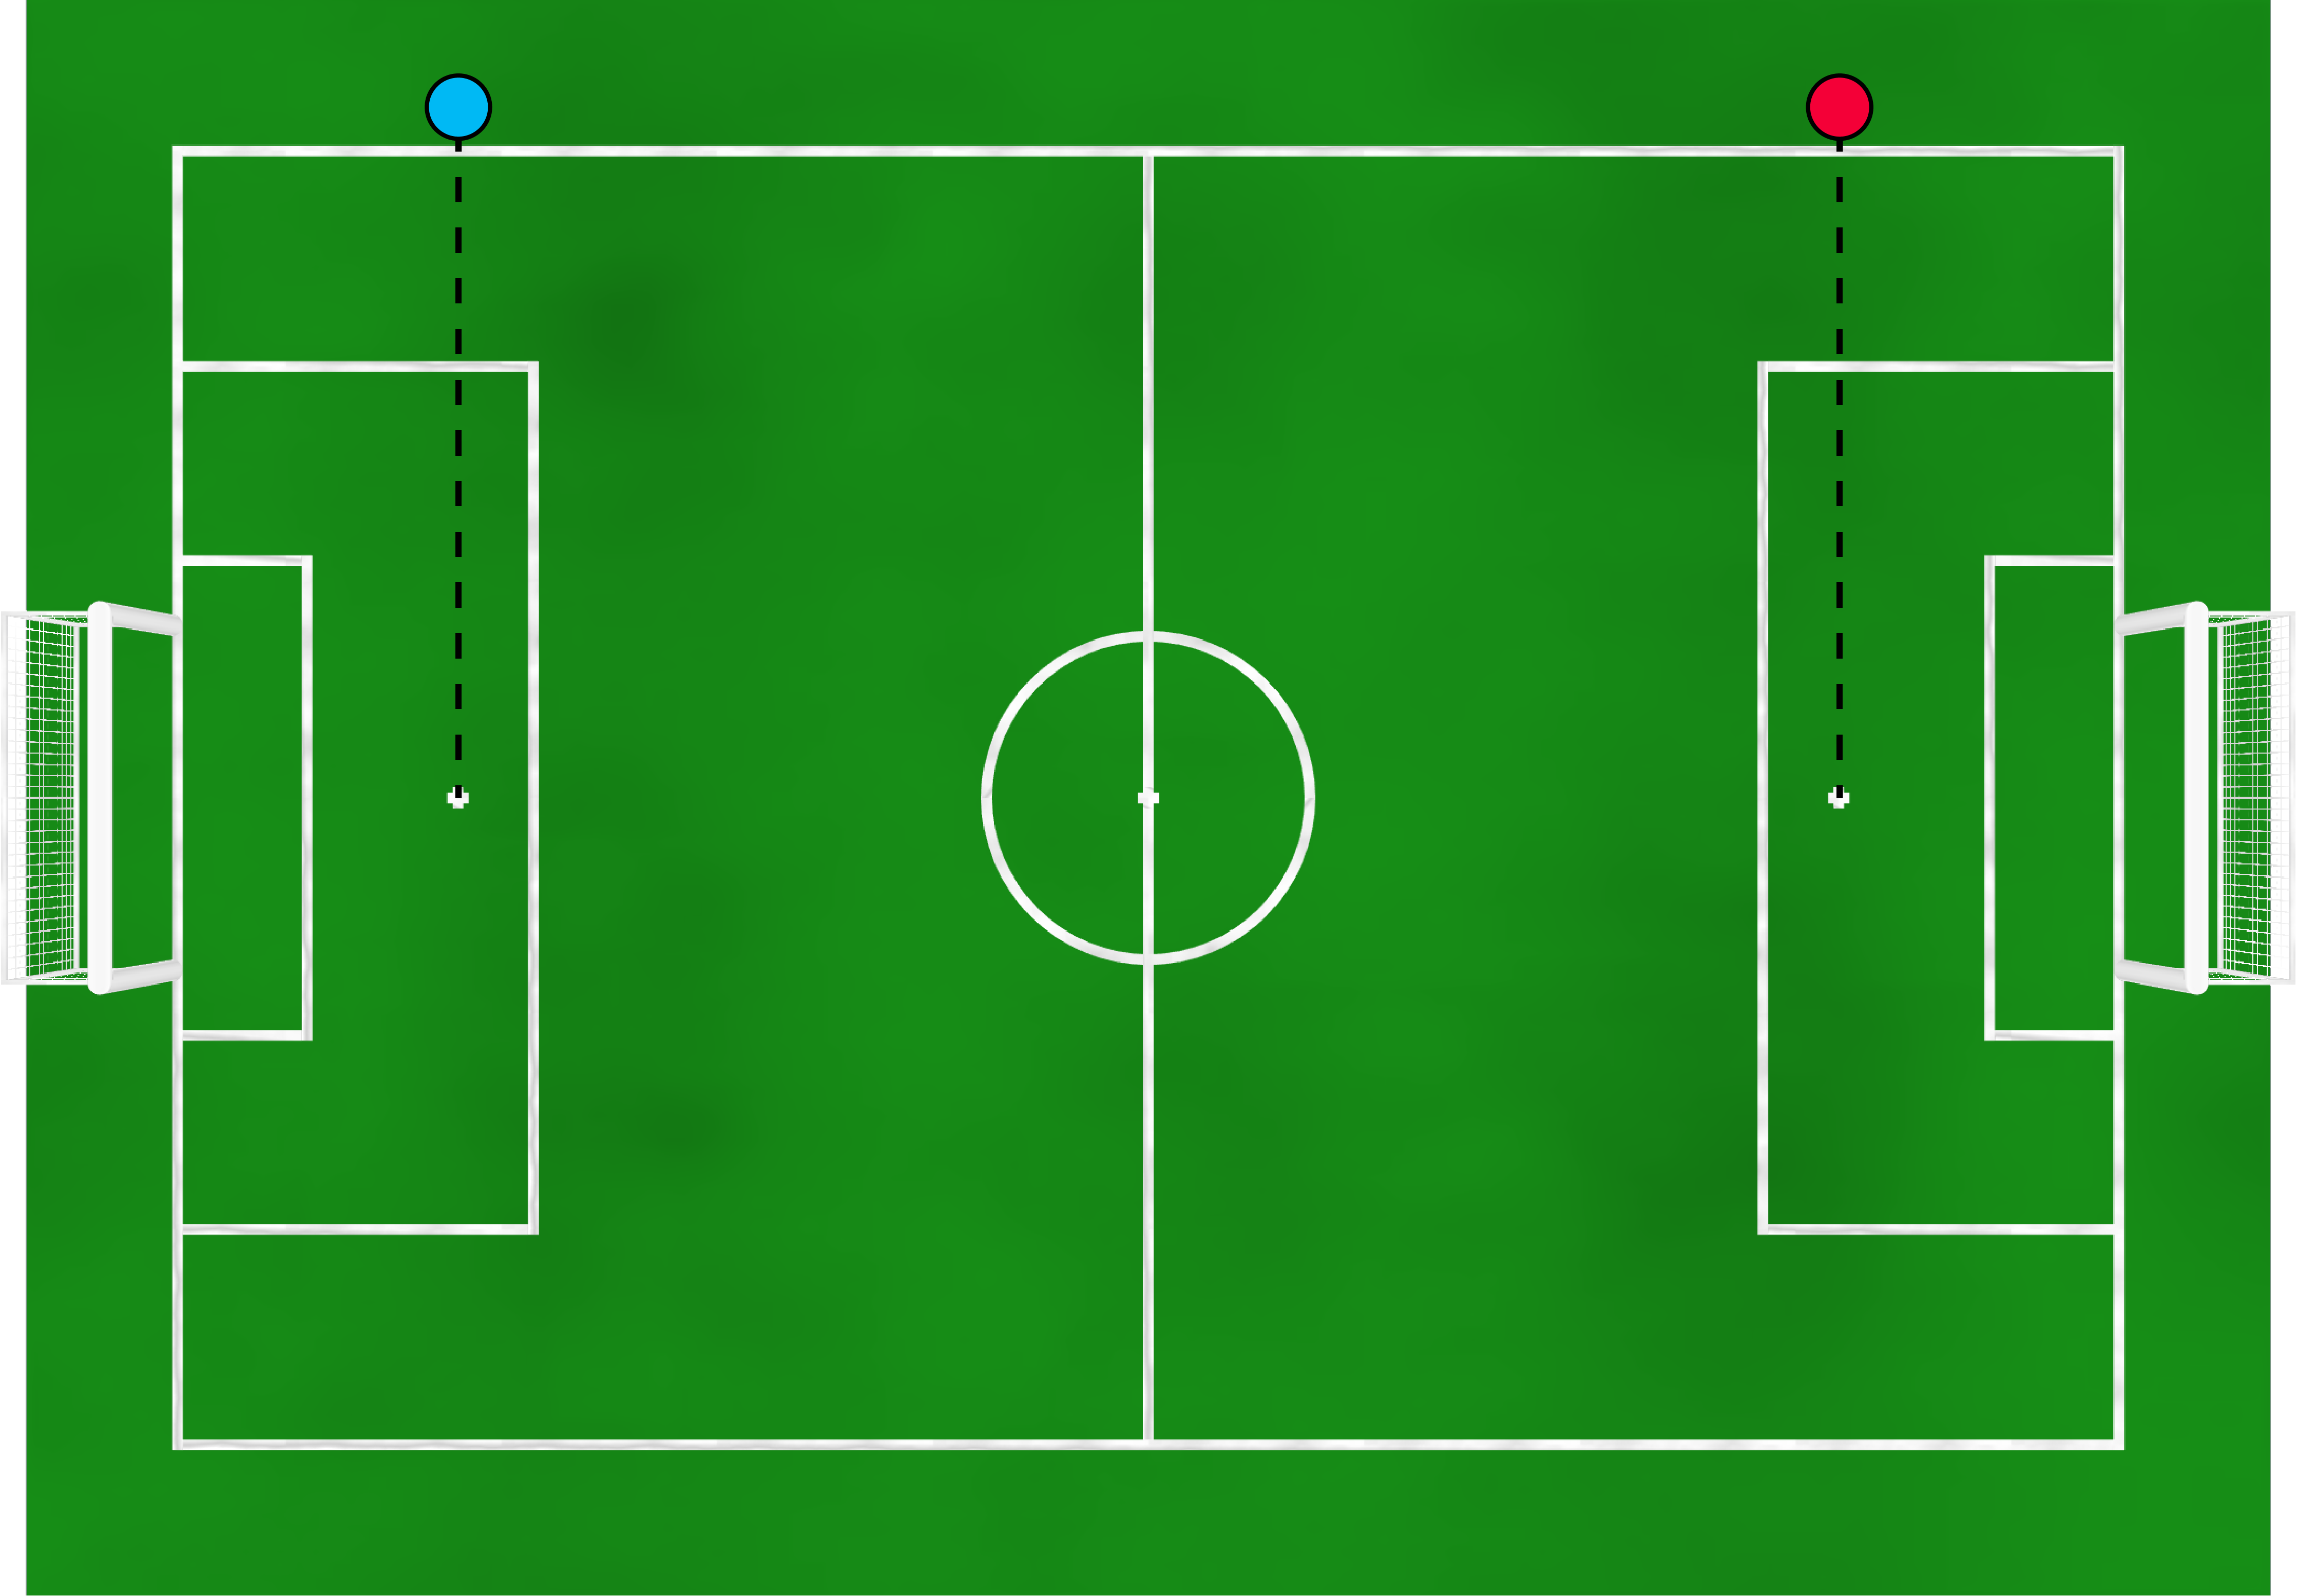
\includegraphics[width=\columnwidth]{figs/penalty_re-entry_points_2020.png}}
	\caption{For robots coming back from a standard removal penalty, re-entry points  are inline with the penalty spot in their own half, on the sideline on the side away from the ball.}
	\label{fig:penalty_re-entry_points}
\end{figure}

When the robot is on the field again, the operator of the GameController will send the \emph{playing} signal to it.

\subsubsection{Forbidden Actions}

The following actions are forbidden, but not treated as penalties.
Each forbidden action specifies the actions to be taken by the referees.

\paragraph{Manual Interaction by Team Members}

Manual interaction with the robots, either directly or via some communications mechanism, is not permitted.

\paragraph{Locomotion Type}
\label{sec:locomotion_type}

Robots should clearly demonstrate bipedal walking similar to human walking. Other types of locomotion involving other parts than feet (crawling etc.) are strictly forbidden.
The head referee decides whether a robot's locomotion is appropriate. Robots using inappropriate locomotion types will be removed via ``Request for Pick-up'' until they are able to show appropriate locomotion.

\paragraph{Damage to the Field}
\label{sec:damage}

A robot that damages the field, or poses a threat to spectator safety, will be removed from the field for the remainder of the game.
%Similarly, a robot that poses a threat to spectator safety will also be removed from the field for the remainder of the game.

\paragraph{Damage to the Robot}
\label{sec:damage}

The head referee decides whether a robot excessively damages itself and will remove it from the field for the remainder of the game.


\newpage
% Arne
All rules from the current rule book apply, except for these changes:

- Refereeing
    - Local team has to referee
    - Referee can prevent robot by crashing on ground if falling by catching it before
    - Team scheidet aus, wenn Laufen so schlecht, dass es zwei Spiele lange nur hingefallen ist

2. The player is only allowed to stay in its own half except between the goal nets. Leaving this area results in a standard removal penalty (leaving the field).
3. play-off-mode in GC?? 
6. Points will be counted by the referees and not by the GC.
7. Points can be scored by:
    - Shooting the ball in opponents half and it stops there (1 Point)
    - Shooting a goal (not own goal) (1 Point)
    - Touching the opponents player with the ball (0 Point)
10. If the score is equal for both teams the game duration gets extended for/by one minute. After each extension the score is evaluated again. At max 5 extensions are allowed. \textcolor{red}{TODO}: Final determination? Coin toss?
11. Teams playing with an autonomous player get a scoring factor of 2. Each point is multiplied by this factor.
12. Dive motions and wide stance is not allowed

\subsection{Challenge execution}
% Arne
- Ladder system
    - KO system 
    - groups of 8 teams per Ladder
    - randomly assignement of teams to groups
    - losers of a match will play in additional ladders (To allow all teams to play at least 3 times)
    - Winners play games against each other
    - Timezones (Two games per day)
    - can only be finalized when the exact number of participants is known